

\documentclass{report}

\usepackage{hyperref}

\usepackage{epstopdf}
\usepackage{amsmath}
\usepackage{amssymb}
\usepackage{subfig}
%\usepackage{multirow}
\usepackage[utf8]{inputenc}
\usepackage[T1]{fontenc}
\usepackage{standalone}
\usepackage{tikz}
\usepackage{tabularx}
\usepackage{float}
\usepackage[section]{placeins}
\usepackage{sverb}
\usepackage{import}
\usepackage{verbatim}
\usepackage{listings}
\usepackage{xcolor}

\graphicspath{{img/}}
\DeclareGraphicsExtensions{.pdf,.png,.jpg,.svg} %For pdflatex






\definecolor{codegreen}{rgb}{0,0.6,0}
\definecolor{codegray}{rgb}{0.5,0.5,0.5}
\definecolor{codepurple}{rgb}{0.58,0,0.82}
\definecolor{backcolour}{rgb}{0.95,0.95,0.92}

\lstdefinestyle{mystyle}{
    backgroundcolor=\color{backcolour},   
    commentstyle=\color{codegreen},
    keywordstyle=\color{magenta},
    numberstyle=\tiny\color{codegray},
    stringstyle=\color{codepurple},
    basicstyle=\ttfamily\footnotesize,
    breakatwhitespace=false,         
    breaklines=true,                 
    captionpos=b,                    
    keepspaces=true,                 
    numbers=left,                    
    numbersep=5pt,                  
    showspaces=false,                
    showstringspaces=false,
    showtabs=false,                  
    tabsize=2,
    float=H,
    extendedchars=\true, 
}


\lstset{style=mystyle}


\begin{document}

\begin{titlepage}
    \begin{center}
        
\includegraphics[width=.50\linewidth]{other/polsl.png}\\
        \Huge
        \textbf{Przetwarzanie Obrazów Cyfrowych}
        \\ \vspace{1.5cm}
        \Large
        \textbf{Raport z ćwiczenia nr. 1: } \\
        % \textbf{WSTĘPNE PRZETWARZANIE OBRAZÓW — FILTRY LINIOWE}
        \textbf{Filtry nieliniowe}        
    \end{center}
    \vspace{3.0cm}
    \Large
    Raport opracował: \\
    Dawid Kania \\
    Grupa 6 Semestr 7 \\ \\
    Data wykonania ćwiczenia: 17.10.2022
\end{titlepage}
 



% \section*{Zadanie}

\newcommand{\ww}{1} 
\begin{figure}[H] 
   \captionsetup[subfloat]{justification=raggedright,singlelinecheck=false, position=bottom,labelformat=empty} % 
    \subfloat[]{
        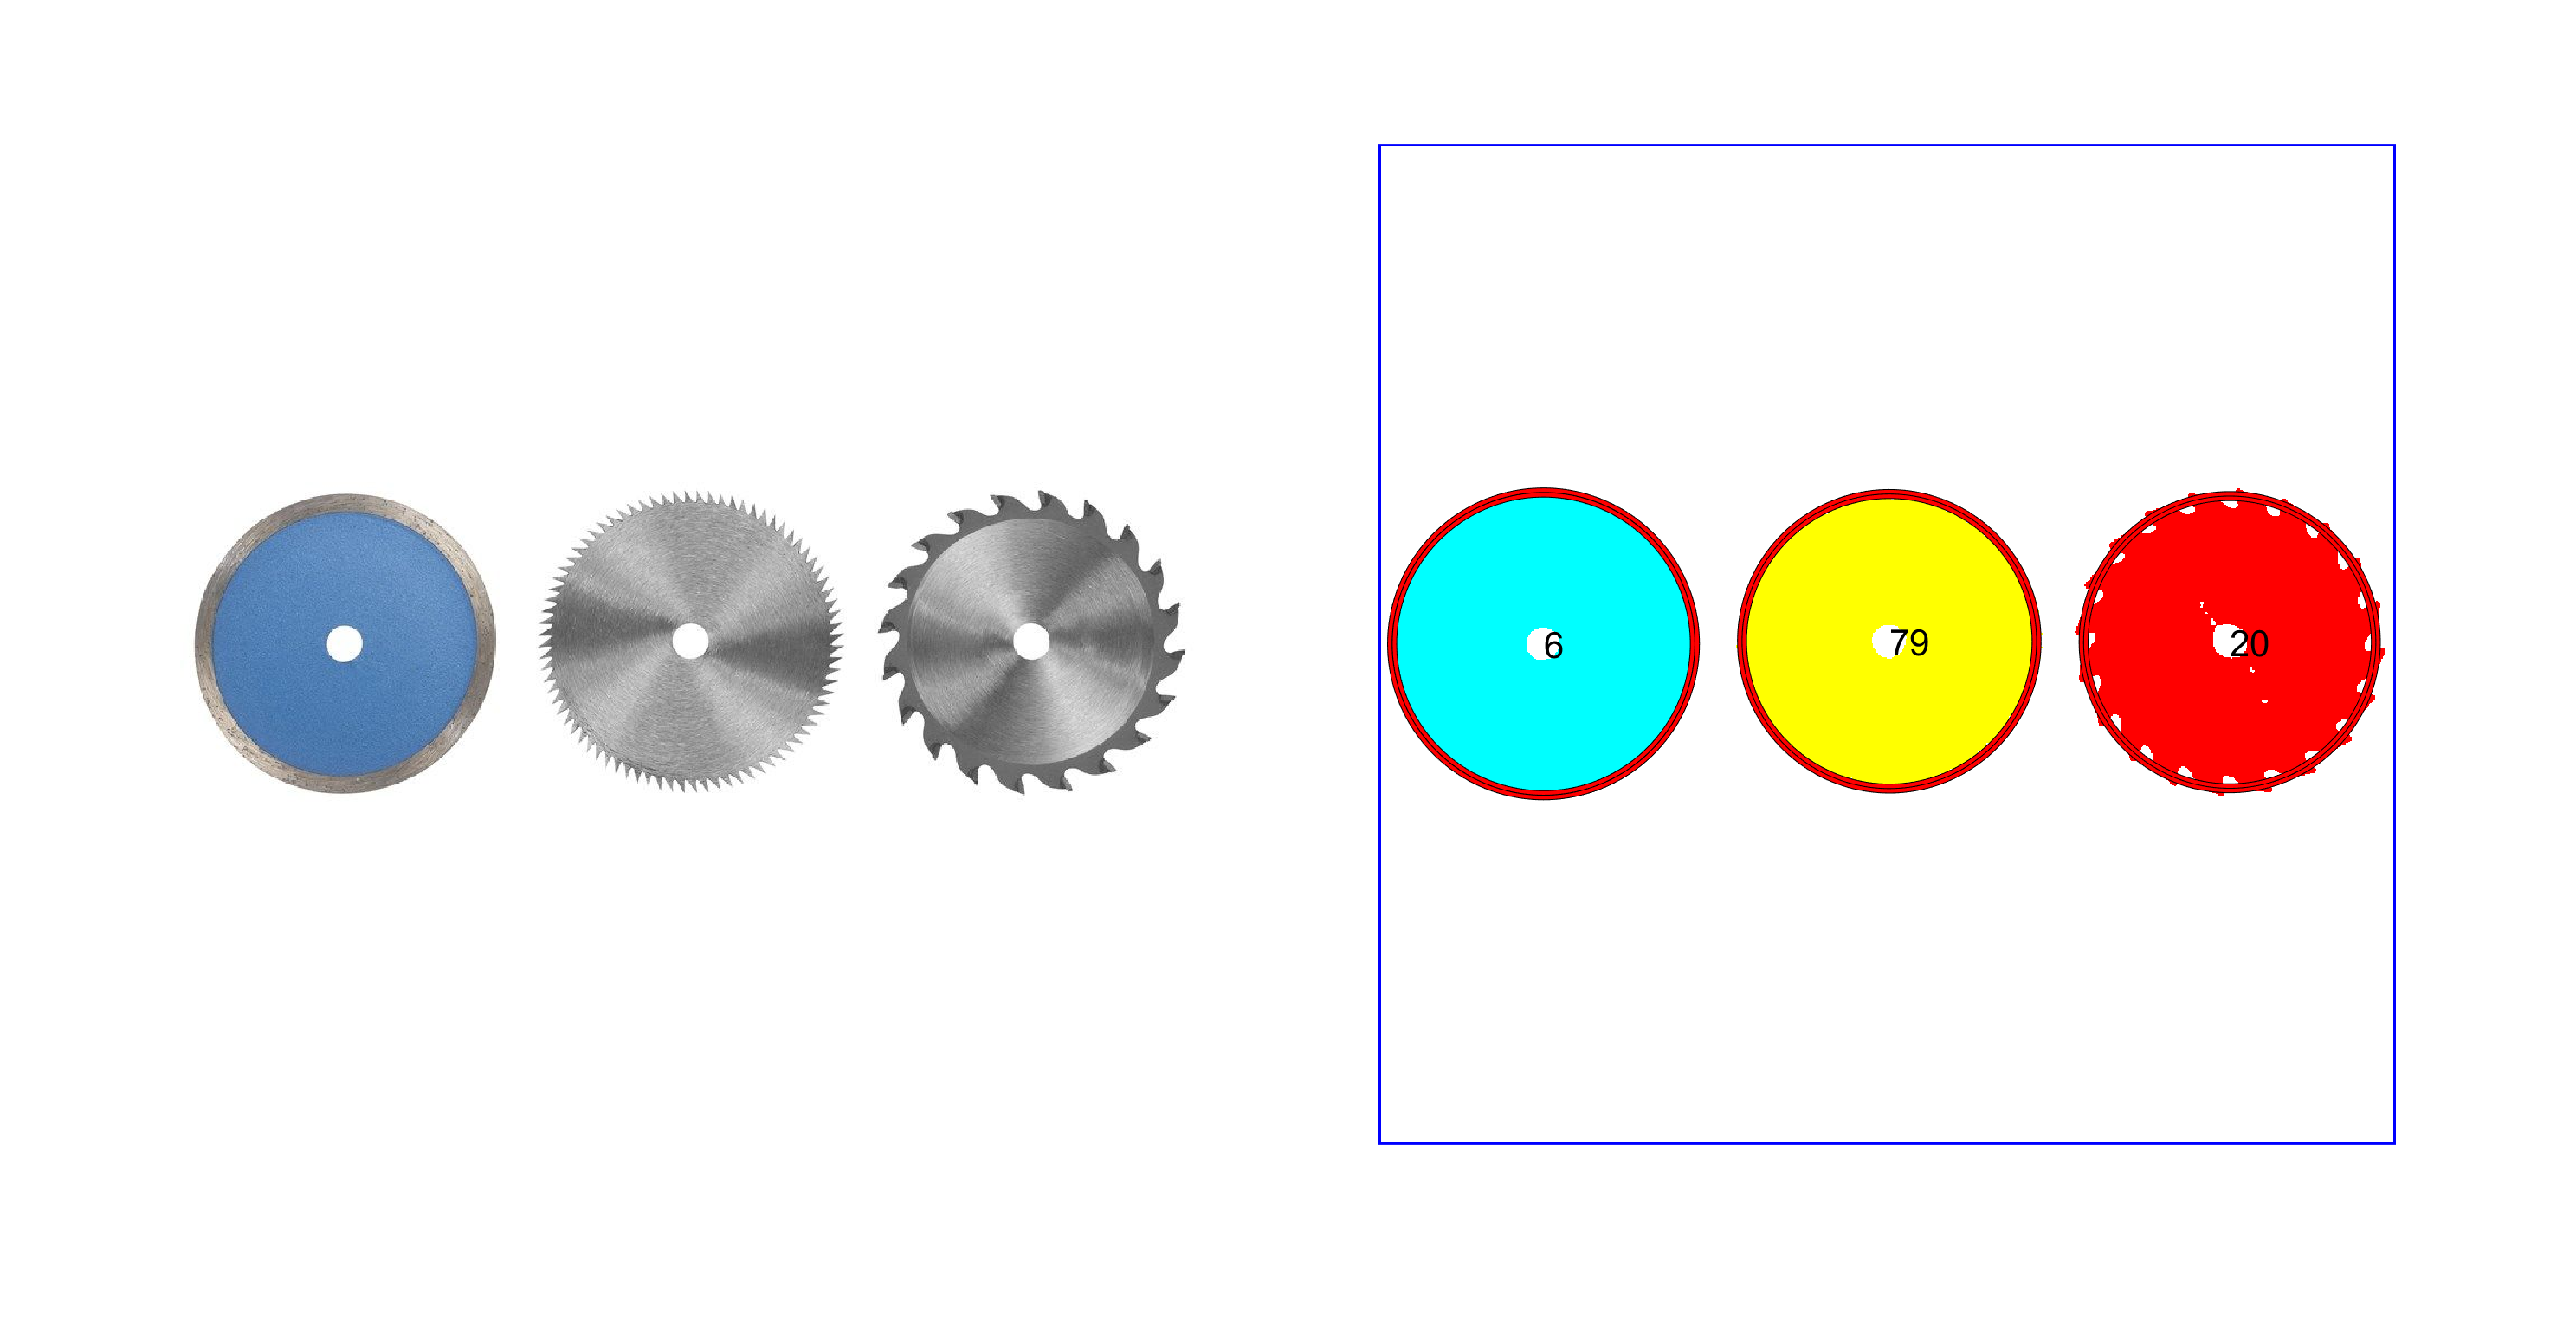
\includegraphics[width=\ww\linewidth]{../result/I.png}}
\caption{Ilość znalezionych zębów}
\end{figure} 

\begin{figure}[H] 
   \captionsetup[subfloat]{justification=raggedright,singlelinecheck=false, position=bottom,labelformat=empty} % 
    \subfloat[]{
        
\includegraphics[width=\ww\linewidth]{../result/I1.png}}
\caption{Znalezione zęby}
\end{figure} 

\begin{figure}[H] 
   \captionsetup[subfloat]{justification=raggedright,singlelinecheck=false, position=bottom,labelformat=empty} % 
    \subfloat[]{
        
\includegraphics[width=\ww\linewidth]{../result/I2.png}}
\caption{Znalezione zęby}
\end{figure} 

\begin{figure}[H] 
   \captionsetup[subfloat]{justification=raggedright,singlelinecheck=false, position=bottom,labelformat=empty} % 
    \subfloat[]{
        
\includegraphics[width=\ww\linewidth]{../result/I3.png}}
\caption{Znalezione zęby}
\end{figure} 
\let\ww\undefined 

\newpage
\section*{Kody programów}
\subsection*{zad1.m}\lstinputlisting[language=Octave]{ "../matlab/zad1.m"} \newpage



\end{document}